% !TEX TS-program = xelatex
% !TEX encoding = UTF-8 Unicode

\documentclass[article,12pt,a4paper,oneside]{memoir}

%\usepackage[top=1in,bottom=1in,right=1in,left=1in]{geometry}

\usepackage{xparse}
\usepackage{etoolbox}
\usepackage{hyperref}
\usepackage{amsmath}
\usepackage{lmelahnDefaultFonts}
\usepackage{longtable,booktabs}
\usepackage{multicol}
\usepackage[xetex]{xcolor}
\usepackage[xetex]{graphicx}
\usepackage{polyglossia}


% Set tables numbering to follow chapters.
% E.g., the second table in chapter three will be Table 3.2
\makeatletter
\@addtoreset{table}{chapter}
\@addtoreset{figure}{chapter}
\makeatother

\renewcommand\thetable{\thechapter.\arabic{table}}
\renewcommand\thefigure{\thechapter.\arabic{figure}}


\definecolor{light-pink}{rgb}{1,0.9,0.9}

\DeclareDocumentCommand{\trueBox}{ +m }{%
  \fbox{#1}%
}
\DeclareDocumentCommand{\falseBox}{ +m }{%
  \fcolorbox{red}{light-pink}{#1}%
}

\providebool{useEnglish}
\providebool{useItalian}
\providebool{useNone}

\makeatletter
\newcommand{\@clearLanguage}
  {
    \boolfalse{useItalian}
    \boolfalse{useEnglish}
    \boolfalse{useNone}
  }
 
\newcommand{\setLanguage}[1]
  { 
    \ifstrequal{#1}{English}
      {
        \@clearLanguage
        \booltrue{useEnglish}
      }{}
    
    \ifstrequal{#1}{Italian}
      {
        \@clearLanguage
        \booltrue{useItalian}
      }{}   
    
    \ifstrequal{#1}{None}
      {
        \@clearLanguage
        \booltrue{useNone}
      }{}   
  }
\makeatother

\providebool{showAnswers}
  \boolfalse{showAnswers}

\NewDocumentCommand{\hideText}{ +m }
  {%
    \ifbool{showAnswers}{{\color{red}\itshape{}#1}}{}
  }

\NewDocumentCommand{\hideRawText}{ +m }
  {%
    \ifbool{showAnswers}{#1}{}
  }

\NewDocumentCommand{\dualText}{ +m +m }
  {%
    \ifbool{useItalian}{#1}{}\ifbool{useEnglish}{#2}{}%
  }

% Set up a question in two alternative languages with answers in each language
\NewDocumentCommand{\answered}{ +m +m +m +m }
  {%
    \dualText{#1\hideText{#2}}{#3\hideText{#4}}%
  }
  
\NewDocumentCommand{\answerBox}{ m }
  {%
    \ifbool{showAnswers}{\fcolorbox{red}{white}{#1}}{#1}%
  }

\setLanguage{None} %Possible values: None, English, Italian

\setLanguage{None}

\ifbool{useEnglish}
  {
    \setdefaultlanguage[variant=american]{english}
  }{
    \ifbool{useItalian}
	  {
         \setdefaultlanguage{italian}
	  }{
	     \setdefaultlanguage[variant=american]{english}
	  }
  }


\ifbool{useNone}{

  
  
  
}{}

\ifbool{useEnglish}{

  
  
  
}{}

\ifbool{useItalian}{

  
  
  
}{}

\begin{document}
    \ifbool{useNone}{
          }{}

    \ifbool{useEnglish}{
          }{}
    
    \ifbool{useItalian}{
          }{} 
          
    \title{A Short Introduction to Logic}
          
    \frontmatter
    \maketitle
    
    \hypertarget{analytic-introduction-to-logic}{%
    \chapter*{Analytic Introduction to
    Logic}\label{analytic-introduction-to-logic}}
    \addcontentsline{toc}{chapter}{Analytic Introduction to Logic}

    If you are reading this text, it is because you are taking a course
    on \emph{logic}. Most of us understand intuitively that logic has
    something to do with thinking correctly, but, because one of the
    goals of this course is to improve our capacity for precision and
    thoroughness in forming our concepts, we will not be satisfied with
    a vague and poorly defined intuition. The question that should
    immediately arise, therefore, is ``What precisely is logic?'' This
    introduction will attempt to give a precise and rigorous answer to
    that question; for that reason, it will need to introduce certain
    ideas from epistemology, metaphysics, philosophical anthropology.
    Although these are not actually part of subject matter of
    logic---the \emph{material object}, as we shall learn to call
    it---they are nevertheless indispensable for learning what logic
    actually \emph{is}. Introducing these topics will also help serve
    one of the reasons why logic is taught at the beginning of
    philosophical studies at all: namely, to lay the groundwork for the
    study of metaphysics.

    {[}Make summary of outline here{]}

    \mainmatter

    \hypertarget{logic-as-a-science-and-and-art}{%
    \chapter{Logic as a Science and and
    Art}\label{logic-as-a-science-and-and-art}}

    \hypertarget{sciences-vs.-disciplines}{%
    \section{Sciences vs.~Disciplines}\label{sciences-vs.-disciplines}}

    Before you read this introduction, chances are that you thought of
    logic chiefly as a \emph{discipline}: that is, as a body of
    knowledge that can be acquired through study. That is not wrong,
    exactly; however, it is limiting. This manner of looking at logic
    considers it only in the abstract---that is, it ignores the
    \emph{being} or the \emph{existence} of logic as it is actually
    found in reality. (In the logic of concepts, we will discuss the
    difference between \emph{abstract} and \emph{concrete} concepts.) In
    fact, this abstract way of looking at a subject is likely how you
    have looked at \emph{all} academic fields, whether that be biology,
    quantum physics, astronomy, psychology, economics, or any other
    course of study. This is a somewhat natural reduction to make,
    because we generally gain access to such fields through formal
    education in a university setting: that is, by taking classes,
    reading books, writing papers, doing laboratory assignments, and the
    like.

    In reality, however, a field of study does not reduce to an abstract
    discipline, a set of propositions that one must acquire. Rather,
    acquiring knowledge in a given discipline produces a real change in
    the mind---or to use more precise terminology, in the
    \emph{intellect}---of the person who learns it. Let me illustrate
    with an example. Consider the following equation:
    \[i \hbar \frac{d}{d t}\vert\Psi(t)\rangle = \hat H\vert\Psi(t)\rangle\]
    Readers familiar with quantum mechanics will recognize this as the
    time-dependent form of the Schrödinger equation.\footnote{The
      equation describes the so-called wave function, which is used to
      determine the probability that a given particle is at a given
      location. Perhaps the most familiar use case is for describing the
      orbitals of electrons about an atomic nucleus.} For unfamiliar
    readers, it is doubtless completely unintelligible. In short, our
    human capabilities alone---in this case our \emph{intellect}, our
    capacity for knowledge of things in themselves---are insufficient in
    order to interpret an equation of this kind. Rather, in order to
    understand it, we would need to undergo a stable change in our
    intellect. The intellect alone and unaided will not serve, but it
    requires a modification or ordering---or, to use the technical term,
    an \emph{habitus}.\footnote{I am going to use the Latin term
      \emph{habitus} so as to avoid confusion with the English word
      \emph{habit}, which primarily refers to an involuntary ``tic'' or
      pattern of behavior. An \emph{habitus} (pronounced with a silent
      initial \emph{H}) is a permanent disposition or ordering of
      something to an end.} Since the intellectual \emph{habitus} in
    question helps us primarily to know things, rather than to do
    things, we will call it a \emph{science}.

    Notice that I have not identified the \emph{science} of quantum
    mechanics primarily with the \emph{discipline}. Rather, the
    \emph{science} of quantum mechanics refers to the permanent and
    stable modification of the intellect, the \emph{habitus} that is
    acquired by studying quantum mechanics. This is not the usual,
    modern usage of the term \emph{science}, but rather, it reflects how
    classical philosophers used it---or rather, ἐπιστήμη
    (\emph{epistéme})\footnote{This term, of course, is the root of the
      word \emph{epistemology}, the study of science or knowledge.} for
    the Greek philosophers, and \emph{scientia} for Medieval thinkers.
    We will follow the classical usage of the term \emph{science} in
    this introduction: an intellectual \emph{habitus} that permits or
    helps us to acquire knowledge. A \emph{scientia} is a real,
    existing, concrete attribute of a person---not merely an abstract
    body of knowledge, or discipline.

    As you can probably tell from the foregoing discussion, logic is
    also a science, an ἐπιστήμη: not merely an abstract set of rules,
    but an actual intellectual \emph{habitus} that exists (in technical
    terms, we say that it is \emph{inherent}) in the logician's very
    person. It will, therefore, be useful to explain in greater detail
    what a science (an ἐπιστήμη) is, and how it is different from other
    \emph{habitus}\footnote{The plural of the Latin word \emph{habitus}
      is also \emph{habitus}.}---and also, how to demonstrate that logic
    is, in fact, a science.

    \hypertarget{the-essential-characteristics-of-any-science}{%
    \subsection{The Essential Characteristics of any
    Science}\label{the-essential-characteristics-of-any-science}}

    Taking its cue from Aristotle's seminal work on epistemology, the
    \emph{Posterior Analytics}, Medieval thinkers have generally
    described science (ἐπιστήμη) as \emph{cognitio certa per
    causas}:\footnote{See \textsc{Aristotle}, \emph{Posterior Analytics}
      (henceforth cited as \emph{PA}), tr. by \textsc{G.R.G. Mure}, I.2,
      71b9-11: ``We suppose ourselves to possess unqualified scientific
      knowledge of a thing, as opposed to knowing it in the accidental
      way in which the sophist knows, when we think that we know
      \emph{the cause on which the fact depends}, as the cause of that
      fact and of no other, and, further, that the fact could not be
      other than it is.''} in other words, what distinguishes a science
    from mere opinion (Greek: δόξα, \emph{dóxa}) is that one is able to
    link the individual facts known to their causes.

    For example---one that is perhaps more familiar to readers than
    quantum mechanics---consider the example of medical science. For
    millennia, humans have been aware that certain diseases are
    contagious. Perhaps the most notorious example is during the Black
    Death in Europe (1347-1351): in order to avoid the spread of the
    disease, those who were infected, or were suspected of being
    infected, were often quarantined\footnote{From the French
      \emph{quarantaine} (``fortyish''), which is ultimately derived
      from the Latin \emph{quadraginta}, forty.}---that is, isolated
    from the rest of society for forty days. In other words, Europeans
    had formed the correct \emph{opinion} regarding the tendency of the
    plague to spread from host to host. However, it was not until the
    advent of the microscope and the development of the germ theory of
    disease (based largely on the work by Louis Pasteur and Robert Koch
    in the late nineteenth century) that the true \emph{causes} of the
    plague became known---and thus effective prevention and treatment
    could be developed. We could say that the study of infectious
    disease did not truly become a \emph{science} until the causes were
    discovered. Similarly, even today, a person might be aware that
    washing one's hands to avoid the spread of infection is a good idea,
    or that antibiotics are an effective treatment against bacterial
    diseases such as the plague, and yet not know that infection by
    bacteria is the \emph{cause}. In that case, the person has the
    correct δόξα, or opinion, regarding these matters, but he does not
    posses ἐπιστήμη.

    Similarly, there is the example of chemistry. For many years,
    scientists were aware that certain chemical species could only
    combine with one in other in certain proportions. For example,
    combining one volume of elemental hydrogen with another volume of
    elemental chlorine would produce, once the mixture had cooled to its
    original temperature, two volumes of hydrogen chloride (hydrochloric
    acid). However, combining two volumes of hydrogen with one volume of
    chlorine would produce a three-volume mixture of 1/3 hydrogen and
    2/3 hydrogen chloride. The reason why the hydrogen remained a
    separate species was a mystery, until the atomic theory was
    proposed, and the existence of molecules (stable combinations of
    atoms) was discovered. In fact, elemental hydrogen and chlorine are
    both constituted by diatomic (two-atom) molecules
    (H\textsubscript{2} and Cl\textsubscript{2}), and when they combine,
    they form molecules with one hydrogen and one chlorine atom (HCl).
    This arrangement explains why some hydrogen remains unreacted: once
    the chlorine is entirely consumed, it can no longer react. In other
    words, the phenomena observed in the laboratory were not
    satisfactorily explained until their \emph{causes} were discovered.

    Although the seeking of causes is what distinguishes science from
    opinion, Aristotle identifies three other essential characteristics
    of a science: namely, it must be \emph{certain}---that is, it must
    lead to true knowledge without fail or error\footnote{As Aristotle
      points out in the text cited above, by seeking the causes of a
      phenomenon, the whole purpose is to ensure that ``the fact could
      not be other than it is'' (\emph{PA} I.2, 71b11), and as a
      consequence, such knowledge is free from error.}; it must study
    that which can be attributed to its object in a \emph{necessary} way
    (i.e., it identifies what cannot possibly be otherwise)\footnote{See
      \emph{PA} I.2, 71b14---15: ``Consequently the proper object of
      unqualified scientific knowledge is something which cannot be
      other than it is.''}; and it must be \emph{universally} applicable
    to its object of study.\footnote{See \emph{PA} I.11, 77a5-9: ``So
      demonstration does not necessarily imply the being of Forms nor a
      One beside a Many, but it does necessarily imply the possibility
      of truly predicating one of many; since without this possibility
      we cannot save the universal, and if the universal goes, the
      middle term goes with it, and so demonstration becomes impossible.
      We conclude, then, that there must be a single identical term
      unequivocally predicable of a number of individuals.''}

    Again, it can help to think of some examples. Consider the science
    of chemistry, which helps us to understand the properties of
    material entities, as regards the interactions that occur on the
    atomic and molecular level. It is clear that chemistry provides a
    great degree of \emph{certainty}: if I mix sodium bicarbonate
    (H\textsubscript{2}CO\textsubscript{3}) with hydrochloric acid (a
    solution of HCl in water), I can be \emph{sure} that table salt
    (sodium chloride, NaCl) and carbon dioxide (CO\textsubscript{2})
    will be produced. Similarly, one way to test to see if I have a
    base, such as sodium bicarbonate, is to mix a little hydrochloric
    acid into it; if it bubbles, I can be \emph{certain} of it. In a
    similar vein, when I mix the acid into the bicarbonate, the outcome
    is the production of salt and carbon dioxide---and this result could
    not possibly be otherwise; that is, the evolution of these products
    is a \emph{necessary} result. Finally, the result is
    \emph{universal}, because it applies to \emph{all} similar
    situations: in short, bicarbonate by nature reacts with hydrochloric
    acid, therefore \emph{all} samples of bicarbonate will react with
    \emph{all} batches of the acid. Another way of saying this is that
    chemistry studies only that which can be attributed \emph{per se}
    (in and of itself) or \emph{essentially} to the entities studied.
    Finally, as I mentioned above, chemistry is a science precisely
    because it seeks to identify the \emph{causes} of these properties
    and reactions, which are to be found fundamentally in the atomic and
    molecular structures of the materials, especially in the arrangement
    and interaction of the electrons about the nuclei of the atoms.

    The degree of certainty and necessity---and thus its universal
    applicability---can vary from science to science. Clearly, the
    degree of certainty and necessity that can be attained in pure
    mathematics is much greater than what can be obtained in a social
    science such as psychology or economics. Nevertheless, even in cases
    in which complete certainty, necessity, or universality are
    unattainable, a science provides useful knowledge \emph{to the
    degree} that it is certain, necessary, and universal. For example,
    economics affirms that by and large (but not necessarily in every
    single case), when the price of a good or service rises, the
    quantity demanded falls. Although economics is unable to predict
    what an individual consumer will do, it does accurately account for
    general trends among many consumers. What a science cannot do is
    account for phenomena that have no essential link to their causes
    whatsoever; that is, science cannot account for what is \emph{per
    accidens} (completely incidental). To a geneticist studying fruit
    flies, for example, what interests him are the laws the govern the
    inheritance of genetic characterists---what the flies happen to eat
    for food does not interest him, as such, since it does not affect
    heredity.

    In summary: a science or ἐπιστήμη is an intellectual \emph{habitus}
    that helps the intellect to understand a given object of study. As
    such, it always has four essential characteristics:

    \begin{enumerate}
    \def\labelenumi{\arabic{enumi}.}
    \item
      Most fundamentally, it seeks to connect the phenomena it studies
      to their underlying causes. The seeking of causes is what
      distinguishes science (ἐπιστήμη) from opinion (δόξα), and the
      other three characteristics of a science all follow from this one.
    \item
      It provides certain knowledge of its object---that is, it enables
      the one who possesses the science to know without error.
    \item
      It accounts for phenomena that cannot be different from the way
      they are, or cannot come about in a different way. That is, it
      accounts for phenomena that are linked necessarily (\emph{per
      se}), and not merely incidentally (\emph{per accidens}), to the
      object of study.
    \item
      Finally, it applies universally to the object of study: there is
      no science, as such, of singulars and particulars.
    \end{enumerate}

    A couple of things follow from this. First of all, in order to
    determine whether a given intellectual \emph{habitus} is a science,
    it is sufficient to show that it has these four characteristics. We
    will revisit this topic below. Second, it is not possible for
    science or ἐπιστήμη, in the strict sense of the term, to be false;
    that is, false information is the result, not of science, but of
    erroneous opinion (δόξα).

    \hypertarget{speculative-vs.-practical-sciences}{%
    \subsection{Speculative vs.~Practical
    Sciences}\label{speculative-vs.-practical-sciences}}

    We are not, however quite through with our examination of science:
    as it turns out, sciences come in different kinds, depending on
    their object of study and method. By now, you may have intuited that
    by defining science as the ancient and Medieval philosophers
    did---as \emph{scientia} or ἐπιστήμη, that is, as an intellectual
    \emph{habitus} whose purpose is to know the properties of a given
    object of study according to its causes---we are including under the
    banner ``science'' many more fields than are customarily placed
    there. By this definition, ``science'' is not limited to empirical
    fields such as biology, chemistry, or physics, but rather includes
    areas of study as diverse as mathematics, metaphysics, theology, and
    ethics. It is sufficient that each field have a specific and unique
    object of study (the \emph{genus subiectum}) and appropriate methods
    for it.

    Sciences can be categorized according to their finality---a
    criterion that is particularly useful for us. In the modern
    parlance, we speak of \emph{pure sciences} such as biology,
    chemistry, and physics, and contrast them to \emph{applied sciences}
    such as medical science and engineering. This division can be
    generalized to apply to all sciences (in the classical sense, as we
    have defined the term here): that is, some sciences seek knowledge
    of their object for its own sake, whereas other sciences seek the
    applications of the knowledge gained from them to some action. In
    the classical terminology, the former are called \emph{speculative
    sciences}, whereas the latter are called \emph{practical sciences}.

    Again, it can be helpful to look at some examples. Consider the
    sciences listed in Table \ref{tab:table1}. What the speculative
    sciences listed in the left-hand column have in common is that they
    all seek knowledge of the object they study for its own sake. For
    example, a biologist can study the behavior of nesting robins
    without having any practical purpose whatsoever. This or that
    scientist may in fact have ulterior designs (he may be thinking of
    starting a business raising robins for their eggs), but that
    ulterior motive (or lack of one) does not change the character of
    his work \emph{as a biologist}. The same can be said for chemistry,
    physics, mathematics, and metaphysics\footnote{In fact, metaphysics,
      the study of being (that is, of \emph{ens}, that which is) as
      being, or being \emph{qua} being, is rightly considered the most
      speculative of all sciences, since it has no direct practical
      application.}.

    \begin{table}[ht]
    \begin{center}
    \caption{A few examples of speculative and practical sciences. As much as possible, each practical science is placed next to the speculative science it is derived from.}
    \label{tab:table1}
    \begin{tabular}{l|l}
    \toprule
    Speculative & Practical \\
    \midrule
    Metaphysics & — \\
    —           & Ethics \\
    Biology     & Medical science \\
    Chemistry   & Chemical engineering \\
    Physics     & Mechanical engineering \\
    Mathematics & — \\
    \bottomrule
    \end{tabular}
    \end{center}
    \end{table}

    On the other hand, the practical sciences listed in the right-hand
    column all have a specific kind of operation (that is, a kind of
    action), in mind. What they produce is still a kind of
    \emph{knowledge}, but in contrast to speculative sciences, for
    practical sciences, knowledge is not an end in itself---it is a
    means to action. For example, studying physics by itself will not be
    enough to tell you how to build a bridge; for that, you would need
    to study mechanical engineering. You need to learn how to apply the
    general principles discovered in physics to the more concrete
    problem of how to build structures. Similarly, studying
    biology---even the human biology---by itself is insufficient to
    discover how to cure disease; that is the task of medical science.
    As you can probably tell from these examples, many practical
    sciences can be pared with a speculative science from which they are
    derived. In a similar vein---although it may not be obvious at
    first---ethics, the study of human actions (actions that involve the
    free choices made by the will) in order to discern whether they are
    right or wrong---is also in the column of practical sciences. This
    is so, because the entire purpose of ethics is to direct our
    actions: we wish to discover which behaviors are compatible with
    human happiness, and which ones are not---in other words, the
    knowledge obtained through ethics is a means to the end of behaving
    well.

    \hypertarget{is-logic-a-science}{%
    \subsection{Is Logic a Science?}\label{is-logic-a-science}}

    It is now time to turn our attention once more to our
    topic---logic---and to apply the principles we have been discussing.
    As we saw above, logic is clearly an academic discipline and field
    of study (at least when taken in the abstract), but the question now
    arises: is logic a \emph{science} like biology, chemistry, and
    mathematics? In order to answer this question, we will need to apply
    our definition: a science is a \emph{cognitio certa per causas}.

    Is logic a \emph{cognitio}---that is, an \emph{habitus}, or stable
    disposition, of the intellect? In other words, in the absense of
    logic, would the intellect be impeded from acquiring certain types
    of knowledge? We will see this more clearly when we give the
    definition of logic below, but even based on our intuitive
    understanding of logic, we can confidently answer ``yes'': in fact,
    in the complete absense of logic, we would be unable to acquire any
    knowledge \emph{at all}---and a systematic study of logic makes our
    thinking easier, more ordered, and less prone to error.

    Does logic provide sure and certain knowledge by linking what it
    studies to its causes? As we will see, the answer is again ``yes.''
    Logic seeks the \emph{causes of knowledge}: for example, through
    logic, I can be sure that conclusion \(C\) follows from premises
    \(A\) and \(B\). This type of causality is different from that
    sought, say, in the sciences I listed above, all of which seek the
    \emph{causes of being}, rather the causes of knowledge. That is, the
    \emph{logical} causality proper to logic is distinct from the
    \emph{ontological} causality proper to other sciences---but it is
    still causality.

    Finally, what about the other essential characteristics of a
    science? Does logic provide \emph{certain} knowledge---that is,
    knowledge without error? Does it supply knowledge that follows
    necessarily from the nature of its object of study? Does the
    knowledge it furnishes apply universally to its object? Again, the
    answer to all three questions is in the affirmative. As regards
    certainty, the very purpose of logic is to facilitate our reasoning
    ability and make it less prone to error. As regards necessity,
    again, logic provides the tools we need to see that the conclusions
    we reach are the correct ones, and could not be otherwise. As
    regards universality, it is clear that logic applies to \emph{all}
    of the works of our intellect, without exception.

    In fact, we should carefully define our terms, here, because there
    are two distinct entities without which knowledge is simply
    impossible: there is our intellect, which is the faculty that
    permits us to make acts of knowledge---knowledge that captures the
    very essence and being of things; and there is the intellectual
    \emph{habitus} that we are discussing here. For this reason,
    intellect, which is sometime called our \emph{reason} (in Latin:
    \emph{ratio}; in Greek: λόγος or \emph{lógos})\footnote{In the
      strict sense, our \emph{reason} refers to our capacity for
      acquiring new knowledge starting from knowledge that we have
      already acquired: that is our ability to infer or draw
      conclusions, or, to use the technical term, our
      \emph{ratiocinium}. However, when taken broadly, the term
      \emph{reason} is synonymous with the intellect.}, can be called a
    kind of ``natural logic.'' However, logic, in the strict sense of
    the term, refers to an \emph{habitus}, an acquired ability that
    \emph{helps} the intellect in its operation. However, it should be
    noted that this logic-as-science can be acquired in an imperfect way
    (that is, the intuitive grasp of logic that we acquire from the mere
    use of our reason), or else in a ``perfect'' or systematic
    way---which is what this course is attempting to do.

    We must, therefore, conclude that logic is indeed a science.

    \hypertarget{logica-utens-vs.-logica-docens}{%
    \subsection{\texorpdfstring{\emph{Logica utens} vs.~\emph{logica
    docens}}{Logica utens vs.~logica docens}}\label{logica-utens-vs.-logica-docens}}

    Based on our previous discussion, the another question arises: is
    logic a \emph{speculative} science or a \emph{practical} science? A
    we saw, the purpose of a speculative science is knowledge for its
    own sake. Logic certainly seems to fit the bill. St.~Thomas Aquinas
    in his \emph{Summa theologiae} describes the purpose of logic in
    this way:

    \begin{quote}
    {[}A{]} certain art is required, one that can direct the very act of
    reason, through which man, if you will, in that same act of reason
    may proceed in an orderly manner, more easily, and without error,
    and this art is logic, that is, the rational science.\footnote{\textsc{Thomas Aquinas},
      \emph{Expositio libri Posteriorum Analyticorum} (henceforth cited
      as \emph{EPA}), proemium 1-2: ``{[}A{]}rs quaedam necessaria est,
      quae sit directiva ipsius actus rationis, per quam scilicet homo
      in ipso actu rationis ordinate, faciliter et sine errore procedat.
      Et haec ars est Logica, idest rationalis scientia'' (my
      translation).}
    \end{quote}

    Thus, the purpose of logic is to order the individual actions of our
    intellect in such a way that the acquisition of knowledge is easier
    and less error-prone. When someone has acquired the science of
    logic, it will be much easier for him to distinguish truth from
    falsehood; in fact, we could summarize Aquinas' description here as
    saying that logic is our instrument for discovering true knowledge,
    and ensuring that it is \emph{true}.\footnote{A reminder that, for
      the ancients, \emph{knowledge} (\emph{scientia}, ἐπιστήμη) as such
      is always true. There can be false \emph{opinion} (δόξα), but not
      false \emph{knowledge}; we will follow that convention in this
      course. (I will also mention that the ancients used the same term
      \emph{scientia} or ἐπιστήμη to refer both to the
      \emph{habitus}---that is, the habitual knowledge that is not
      necessarily in act---and to the individual \emph{acts} of
      knowledge that flow from the \emph{habitus}.)} As such, we can
    categorize logic as a speculative science, albeit a unique one,
    because (as we will see) its ultimate goal is not knowledge of its
    object---the works of reason---but rather knowledge of the objects
    of all the \emph{other} sciences. That is, we do not study logic in
    order to study the works of reason for their own sake; rather, we
    study the works of reason in order to \emph{use} them in biology,
    mathematics, physics, engineering, and every other science
    (including logic itself)---indeed in every act of the intellect. We
    can summarize this idea by saying that logic is \emph{instrumentally
    speculative}: it certainly seeks knowledge for its own sake, but it
    does so strictly \emph{as a means or instrument} of obtaining that
    knowledge.

    A new question immediately arises: if logic is a means to obtaining
    knowledge, and obtaining knowledge is an action, doesn't that make
    logic a practical science? It does indeed. What this means is
    that---somewhat surprisingly---``speculative'' and ``practical'' are
    not mutually exclusive: a science can be both.

    How is this possible? It goes back to what we touched on earlier: a
    science, being an intellectual \emph{habitus}, makes it possible for
    the intellect to do certain actions that it was unable to do before.
    An \emph{habitus} is only required when there is a special
    difficulty in acquiring the knowledge in question: for instance
    (referring to the example above), I only need to learn (that is,
    acquire habitual knowledge of) quantum physics if I need to
    understand things like the Schrödinger equation. As we discussed
    above, many speculative (``pure'') sciences can be pared with a
    practical (``applied'') science---for instance, mechanics (physics)
    with mechanical engineering, or human biology with medical science.
    Why is a distinct applied science necessary? In short, because the
    application is not always obvious: mechanics, for example, tells me
    how to calculate the forces acting on a rigid body; it does not tell
    how to apply this knowledge to building a bridge. Similarly, human
    biology tells me that cancers are caused by genetic mutations that
    accumulate in the DNA of the body's cells; it does not tell me the
    best \emph{treatment} for removing that cancer. In sum: when the
    application of speculative knowledge poses a particular difficulty,
    a distinct \emph{habitus} (in this case, a distinct \emph{science})
    is required in order to make that application.

    With logic, however, the situation is a bit different. Since logic
    studies the very works of our reason and (as we will see) the proper
    construction of relations between them, merely studying the object
    of logic immediately hones our ability to reason. We will return to
    this idea below.

    In any case, it is clear that, in addition to being a speculative
    science, logic is also a practical science: although logic is
    speculative insofar as its end goal is knowledge, its manner (or
    \emph{mode}) of achieving that goal is practical: said in other
    terms, logic teaches us \emph{how to know}. For this reason, logic
    is said to be a \emph{modally practical} science.

    \hypertarget{is-logic-also-an-art-ux3c4ux3adux3c7ux3bdux3b7}{%
    \subsection{Is Logic Also an Art
    (τέχνη)?}\label{is-logic-also-an-art-ux3c4ux3adux3c7ux3bdux3b7}}

    Attentive readers will note that Aquinas, when describing the goals
    of logic, does a curious thing: he calls it an \emph{art}
    (\emph{ars}; in Greek: τέχνη or \emph{téchne}). That is surprising,
    because we have just spent the last few pages demonstrating that
    logic is a \emph{science}. It may also surprise readers that Aquinas
    calls it an ``art'' along with painting, music, sculpture, and
    theater. In order to understand this, it is best to take a moment to
    understand what Aristotle and Aquinas meant by \emph{art} or
    τέχνη.\footnote{From the Greek word τέχνη, we derive a number of
      English words, including \emph{technique} and \emph{technology}.}

    For Aquinas, an art could refer to any intellectual \emph{habitus}
    that results immediately in action: in the classical formulation,
    \emph{recta ratio factibilium}, right reason applied to things that
    are made. In other words, it is a use of reason or the intellect
    (\emph{ratio}) that is properly ordered (\emph{recta} or ``right'')
    to the accomplishment of determined operations or actions
    (\emph{factibilium}).

    Again, some examples are helpful: suppose you are given a piece of
    marble, and instructions to carve it into a statue of David. For the
    vast majority of readers, the result would most likely not look
    anything like Michelangelo's famous statue of David. As we saw
    before with the sciences, in order for the sculptor to be able to
    set chisel to stone and produce a work of beauty, he must first
    acquire an \emph{habitus}---in this case the art of sculpture. I
    think it is clear that the same reasoning applies to a violinist, an
    opera singer, a painter, and a photographer. However, for Aquinas,
    \emph{art} is not limited to what we would call the ``fine arts'';
    it applies to any \emph{habitus} that is necessary for skilled
    action. Therefore, surgeons, architects, athletes, lawyers,
    carpenters, writers, orators, accountants, and entrepreneurs are all
    ``artists'' by this definition.

    Notice that arts can easily be distinguished by the kind of action
    they produce. Some arts, called the \emph{mechanical arts}, produce
    something that is external: for example, the art of painting results
    in physical artwork such as a fresco or canvass, and carpentry
    results in woodwork such as tables and chairs. On the other hand,
    the \emph{liberal arts} produce something that is internal to the
    intellect: for instance, the art of practicing law does not leave a
    physical work, but rather produces intangibles such as legal
    precedents, decisions, motions, and verdicts.

    As with the sciences, arts have certain characteristics in common.
    Let us take, for example, the art of carpentry. A carpenter takes a
    raw material---in this case, wood---and fashions it into finished
    products, such as tables and cabinets. In order to do so, he applies
    the techniques that he has learned: how to cut, trim, and smooth out
    the wood, putting the pieces together and gluing them in the right
    way, adding the right kind of finish, and so on.

    We can generalize this idea to every art: the practitioner of an art
    takes some indeterminate entity---its ``raw material''---something
    that \emph{can} be fashioned as desired, but \emph{need} not be. He
    transforms it using means that are determined and universal, so as
    to produce the desired product. That is, we could say that, in
    general, an artist's task is to take an indeterminate ``matter'' and
    remove its indetermination. For instance, when Michelangelo
    Buonarotti was given blocks of marble, the number of possible
    statues he could make from them was infinite; it was fully
    \emph{indeterminate}. However, the more he worked on them, the
    closer they became to being fully \emph{determinate}: say, a Pietà.

    In fact, any \emph{habitus} with these two characteristics can be
    classified as an \emph{art} or τέχνη. With the mechanical arts it is
    easy to see, but the same holds for all of the liberal arts: a
    defense lawyer must take all of the facts of the case and his
    knowledge of the laws to formulate a cogent defense for his client;
    an orator must take the infinite possibilities of a language and
    formulate a beautiful speech; a composer must take tones, rhythms,
    dynamics, and instrumentation, and form a musical composition.

    So, what about logic? Could logic be classified as one of the arts?
    To summarize what we saw just now, an \emph{habitus} is an art if it
    fulfills the following characteristics:

    \begin{enumerate}
    \def\labelenumi{\arabic{enumi}.}
    \item
      It takes an indeterminate matter that does not infallibly attain
      its fully determined form.
    \item
      It transforms that matter into a finished product using
      determinate and universal means.
    \end{enumerate}

    \noindent Does logic qualify? (1) Regarding the first condition, as
    we shall see, the task of logic is to take the works of our reason
    (concepts, enunciations, and arguments) and to construct relations
    between them according to very strict and determined rules. Even
    though our reason is ordered to the truth, there is nothing
    preventing us from getting the relations between them incorrect:
    that is, we can fall into error and falsehood. Therefore, these
    works of reason constitute the \emph{indeterminate matter} of logic.
    (2) Regarding the second condition, among all of the possible
    relations among the works of our reason, logic constructs---using
    \emph{universal and determined rules}---the \emph{correct}
    relations, the ones that will produce \emph{true} knowledge. It
    follows that logic is indeed an art: a liberal art, evidently, as it
    does not produce a external product.

    \hypertarget{how-logic-manages-to-be-all-three-at-once}{%
    \subsection{How Logic Manages to Be All Three at
    Once}\label{how-logic-manages-to-be-all-three-at-once}}

    I just want to finish this section with a few more observations
    about the different \emph{habitus} that we have been discussing.
    Ordinarily, speculative sciences, practical sciences, and arts can
    be clearly distinguished from one another, even when their subject
    matter is closely related. Continuing the example I mentioned above,
    human biology is the speculative science at the root of all medical
    matters; medical science is the practical science that applies the
    knowledge of human biology to the treatment of disease; and medicine
    is the art that applies medical science to concrete acts of
    treatment. Three distinct \emph{habitus} are at play here, because
    neither of the two applications is trivial. A surgeon, for example,
    can hardly expect to be sufficiently trained simply by acquiring the
    speculative science of human biology. In fact, not even detailed
    knowledge of medical science is enough: he can spend years learning
    \emph{how} surgeries are done, and yet be completely unprepared for
    performing an actual surgery. In short, he does not become a surgeon
    without first acquiring the art of surgery---which in this case
    implies not only speculative and practical knowledge, but also a
    training in the coordination of the hands. In other words, what
    renders the three \emph{habitus} distinct from one another is that
    there is, if you will, a considerable gap to close between the
    speculative science and the practical science, and between the
    practical science and the art.

    With logic, however, we use our intellect to study works produced by
    that same intellect. Therefore, the distance that is present in
    other fields is absent in logic. We have already noted above that
    the speculative aspect of logic, as a science, cannot be really
    distinguished from its practical aspect. It is also clear from our
    discussion of arts that the \emph{art} of logic cannot be really
    distinguished from the \emph{science} of logic. In other words,
    formal, scientific instruction in logic---what is traditionally
    called \emph{logica docens}\footnote{From the Latin \emph{doceo},
      ``to teach.''}---being the study of an object that is intrinsic to
    the very intellect that studies it, results immediately in an
    improvement in the exercise of logic---what is traditionally called
    \emph{logica utens}\footnote{From the Latin \emph{utor}, ``to use or
      employ.''}. Later on in the course, you will learn to distinguish
    and relate different kinds of concepts, how to relate enunciations
    to one another, and how to form and analyze syllogisms. You will be
    able to use those skills immediately; there is no need for an
    \emph{additional} science, nor for a distinct \emph{art}, in order
    to apply them.

    In sum: we conclude from the foregoing discussion that logic is
    simultaneously an instrumentally speculative science, a modally
    practical science, and an art, whose object is the works of our
    reason. What remains to discuss in greater detail, therefore, is the
    \emph{object} of logic, which we will do after a brief discussion of
    some key concepts in philosophical anthropology that are helpful for
    understanding what we have just gone over.

    \hypertarget{a-primer-on-the-metaphysics-of-man}{%
    \chapter{A Primer on the Metaphysics of
    Man}\label{a-primer-on-the-metaphysics-of-man}}

    In this chapter, we will explore some of the essentials of
    philosophical anthropology: the philosophical, or metaphysical,
    study of mankind.\footnote{We call it \emph{philosophical}
      anthropology to distinguish it from \emph{cultural} anthropology,
      which is empirical, rather than philosophical, in nature.} We will
    do this for two reasons. First of all, although this course is
    designed primarily to study logic, it is also intended to be the
    reader's first exposure to some of the terminology and ideas that
    will form the basis of their philosophical inquiry: for example,
    \emph{ens}, \emph{substance}, \emph{accident}, \emph{faculty},
    \emph{habitus}, and \emph{operation}. Second, by laying the
    philosophical bases, it will be much easier to understand the next
    chapter, in which we discuss what the \emph{object} of a faculty or
    \emph{habitus} is in general, and explain in detail the object of
    logic in particular.

    \hypertarget{what-are-metaphysics-and-anthropology}{%
    \section{What are metaphysics and
    anthropology?}\label{what-are-metaphysics-and-anthropology}}

    Before beginning in earnest, since this is likely the reader's very
    first exposure to the sciences of metaphysics and philosophical
    anthropology, a short introduction to what we are talking about is
    in order.

    \emph{Metaphysics} is the study of anything that exists---of
    \emph{entities} (in Latin: \emph{entia}), as we will call them---not
    according to this or that particular aspect, but simply
    \emph{because they are}. That is, according to Aristotle's famous
    definition, metaphysics is the study of existing things
    (\emph{entia}) \emph{qua} being.\footnote{As Aristotle states in
      \emph{Metaphysics}, ``There is a science which studies Being
      \emph{qua} Being, and the properties inherent in it in virtue of
      its own nature. This science is not the same as any of the
      so-called particular sciences, for none of the others contemplates
      Being generally \emph{qua} Being; they divide off some portion of
      it and study the attribute of this portion, as do for example the
      mathematical sciences. But since it is for the first principles
      and the most ultimate causes that we are searching, clearly they
      must belong to something in virtue of its own nature''
      (\textsc{Aristotle}, \emph{Metaphysics} {[}henceforth cited simply
      as \emph{Metaph.}{]}, tr. by \textsc{W.D. Ross}, Oxford, Clarendon
      Press, 1924, Γ, I.1, 1003α21-28).

      \par

      In languages, like English, that do not distinguish well between
      \emph{being} in the sense of ``something that exists'' (in Latin:
      \emph{ens}) and \emph{being} as a synonym of ``to be'' (in Latin:
      \emph{esse}), this definition is often translated as ``being
      \emph{qua} being'' or ``being as being.'' However, this rendition
      is rather misleading: metaphysics studies existing \emph{things}
      (\emph{entia}) insofar as they are, not primarily that perfection
      or attribute of existing things that we call ``being''
      (\emph{esse}).} We saw above that sciences study their object with
    the goal not only of understanding its properties, but with the hope
    of tracing those properties all the way back to their causes. As can
    be seen, metaphysics is the most general of sciences: no created
    entity is excluded from it whatsoever. Therefore, unlike other
    sciences, it seeks the properties that can be attributed to
    \emph{all} entities without exception,\footnote{We will touch on
      some of these, as they regard logic, when we go over the
      \emph{transcendentals} in the part of the course on the logic of
      the concept.} and it seeks the causes on which \emph{all} things
    depend. It should be noted that metaphysics studies \emph{created
    entities}, and thus God is actually \emph{not} the object of this
    science. Rather, He is of interest as both the First and Ultimate
    extrinsic Cause of all entities:\footnote{Thus, God is not a mere
      entity, in the strict sense of the term, not a mere thing that
      exists: rather, He is Being Itself (Latin: \emph{Ipsum Esse}).}
    the First Efficient and Exemplary Cause, and the Ultimate Final
    Cause.\footnote{This pattern---that the cause is not the object of a
      science---is common throughout all sciences. For example, consider
      biology, whose object is living things as regards their bodily
      life. Biology links the life processes of living things to their
      chemical causes: for example, the chemical pathways by which
      organisms extract the energy in the food they eat helps to explain
      their diets and eating habits. Biology, as such, studies the
      \emph{organisms} and their properties, not the chemical causes of
      those properties; however, of course it relies a lot on the
      findings of chemistry to understand those properties in greater
      depth. In a similar way, the task of metaphysics is to study
      created entities, not God; but knowing something about God helps
      the science considerably in its understanding of entities.}

    Aristotle called this science various names, including the ``first
    Science,'' ``theology'', and ``wisdom''---but not ``metaphysics.''
    That name was given first by the compilers of Aristotle's works
    located in Alexandria, Egypt, simply because they placed those
    treatises \emph{after} Aristotle's works on physics (in Greek: µετὰ
    τὰ φύσικα, \emph{metà tà phýsica}). Despite the trivial origin of
    the name, by an accident of the Greek language, it is actually quite
    appropriate: µετά can also mean ``beyond,'' and it turns out that
    metaphysics is the only philosophical discipline that can transcend
    \emph{beyond} the physical (that is, the material) world.

    When metaphysical principles and findings are applied to mankind,
    the resulting science is \emph{philosophical anthropology}, which
    could be defined as the study of man, not merely regarding this or
    that aspect of man, but \emph{insofar as he is}, or \emph{insofar as
    he is man}. Like other applications of metaphysics, philosophical
    anthropology seeks to find the properties that apply universally to
    its object, man, and links them to their ultimate intrinsic and
    extrinsic causes (that is, man's constitutive metaphysical
    principles, and God as First and Ultimate extrinsic Cause.) For our
    purposes, it will be enough to look at some of the intrinsic causes
    of man---that is, some of the metaphysical principles that
    constitute him.

    \hypertarget{entities-entia-substances-and-accidents.}{%
    \section{\texorpdfstring{Entities (\emph{Entia}), Substances, and
    Accidents.}{Entities (Entia), Substances, and Accidents.}}\label{entities-entia-substances-and-accidents.}}

    The first notion that we will introduce is \emph{ens} (or its plural
    in Latin \emph{entia}), which is the term that classical and
    Medieval philosophers used to translate Aristotle's τὸ ὄν, the
    present participle of the Greek verb εἰμί (``to be''). In English,
    we will be translating \emph{ens} as ``entity.'' As we discussed
    above, an entity is simply something that is, or (in modern
    parlance) exists\footnote{In metaphysics, there is actually a
      difference in meaning between \emph{existence} (Latin:
      \emph{exsistentia}; in later Latin \emph{existentia}, literally
      ``a coming forth'') and \emph{being} (\emph{esse}). Aristotle uses
      the terms τὸ ὑπάρχειν (\emph{to hypárchein}) and τὸ εἶνια
      (\emph{to eînai}) to render the same idea. \emph{Existence} is the
      mere fact that something is, whereas \emph{being} refers to the
      ontological perfection that renders existence possible. Although
      in modern parlance, the terms have come to be practically
      interchangeable, in Aristotle and St.~Thomas Aquinas, they
      maintain their distinct meaning. Thus, as in most cases I am
      referring to being as a perfection, I will try to use the verb
      \emph{to be} as much as possible when referring to entities.}: as
    Aquinas puts it, \emph{id quod est}, ``that which is.'' Aquinas
    actually employs an even more precise description: \emph{id quod
    habet esse} (``that which has being''), which emphasizes the fact
    that the term ``being'' (\emph{esse}) refers to a perfection of the
    entity in question---a reality that is constitutive of that
    entity---not a mere logical fact.

    It should be evident that, outside of God, who is a special case (He
    is not an entity exactly, but is best characterized as Being Itself,
    \emph{Ipsum Esse}), anything that \emph{is} at all, in any way, is
    an entity. That is, there are nothing but entities---anything else,
    simply is not (does not exist). But what counts as an \emph{ens}?
    Let us suppose that there is an oak tree growing in the back yard.
    Since the oak tree clearly \emph{is}, no one can doubt that it is an
    entity (\emph{ens}). However, the oak tree does not merely ``be,''
    as if being could occur in isolation; it has \emph{attributes} and
    properties. For example, it has a height, a width, a weight, a
    place, textures, colors, a time, and a configuration (among many,
    many others). Are these attributes themselves entities
    (\emph{entia})? The answer is not as obvious, since these attributes
    are so closely linked to their substrate, or underlying subject, the
    oak tree. Nevertheless, we can resolve the issue the way Aristotle
    did: since each attribute can be predicated of the oak tree using
    the verb \emph{to be}, it is a sign that we intuitively grasp that
    these attributes enjoy a certain type of being. The height of the
    tree, for example, certainly exists (more precisely, it \emph{is}),
    for if there \emph{were} no height, it would be a very strange tree
    indeed. On the other hand, the attributes of the tree hardly enjoy
    the same kind or degree of being as the tree itself. The oak tree is
    independent, it is ``by itself'' and ``on its own''---or as we say
    in metaphysical terminology, it \emph{subsists}. In contrast, the
    attributes do not exist ``on their own''---it would be absurd to
    think of height, color, weight, or any of the examples given above,
    without some material body to which they correspond---but rather
    they are always ``in'' another entity, or as we say, they
    \emph{inhere} or are \emph{inherent} in another entity.

    By this reasoning, we have discovered the first and easiest division
    of entities: some entities, which we will call \emph{substances}
    (Greek: αἱ οὐσίαι) are \emph{subsistent}, that is, they exist by
    themselves. Others, which we will call \emph{accidents} (Greek: τὰ
    συμβεβηκότος,\footnote{Readers familiar with classical Greek will
      note that Aristotle's term is derived from the preposition σύν
      (``with''), used as a prefix, and the verb βαίνο ``to step or
      walk''---hence the verb συμβαίνο ``to walk alongside.'' The form
      τὰ συμβεβηκότος is the perfect participle.} \emph{ta
    symbebekótos}, literally, ``things that have walked alongside'') are
    mere attributes or modifications of a substance---as we say, they
    are merely \emph{inherent} in a substance. Although substance and
    accident can, in a sense, be thought of logically as the different
    ``types'' of entities, they are best thought of as constituent
    principles of a thing: the oak tree has an intrinsic principle that
    makes it an oak tree---the substance, or, in this context, more
    often referred to as the \emph{essence}---and a set of distinct
    principles, also intrinsic, that give the tree its various
    perfections, such as height, weight, location, and the like.

    At this point, it is appropriate to make a note about the term
    \emph{substance} (Latin: \emph{substantia}), which can take on
    slightly different, but closely related meanings depending on the
    context. At the beginning, when we distinguished substance and
    accident as different kinds of \emph{entia}, we were considering
    substances as fully constituted wholes: for instance, an oak tree,
    including all of its perfections or attributes. Medieval
    philosophers sometimes used the term ``supposit'' (Latin:
    \emph{suppositum}, Greek: ὑπόστασις, \emph{hypóstasis}) to denote
    this meaning of the term \emph{substance}. As we just saw, however,
    \emph{substance} can also be thought of as an intrinsic constitutive
    principle that is composed with the accidents; Western European
    philosophers have generally used the term \emph{essence} (Latin:
    \emph{essentia}) to denote this usage. The two meanings are so
    closely related that Aristotle uses the very same word, οὐσία, for
    both.

    Regardless of how we are using the term \emph{substance}---either as
    supposit or as essence---it is always the answer to the question
    ``What is it?'' Only substances subsist, and thus, only they
    constitute a full answer to this question. As Aristotle clarifies,
    unlike the accidents, only substance constitutes what a thing is
    simply \emph{because} it is (τὸ τὶ ἦν εἶνια, \emph{to ti ên
    êinai})---not because of some perfection or attribute.

    In sum: all created realities (which includes everything with which
    we have habitual contact) are rightly called \emph{entia} or
    entities, because they \emph{are}. Substances are the only entities
    to \emph{subsist}, or be ``by themselves,'' and thus they are
    entities par excellence. Substances are constituted by an intrinsic
    principle, called the \emph{essence}, that gives each substance its
    definition (that is, the essence makes that substance what it is),
    and the essence is composed with various perfections or attributes
    called \emph{accidents}. Entities are always real; anything that
    lacks being entirely is \emph{not} properly called an entity. (This
    idea will become important below, when we talk about \emph{entia
    rationis}.)

    \hypertarget{the-intrinsic-composition-of-man-faculties-habitus-and-operations}{%
    \section{\texorpdfstring{The Intrinsic Composition of Man:
    Faculties, \emph{Habitus}, and
    Operations}{The Intrinsic Composition of Man: Faculties, Habitus, and Operations}}\label{the-intrinsic-composition-of-man-faculties-habitus-and-operations}}

    For the moment, that is enough of an introduction to intrinsic
    metaphysical principles to begin to apply them to our subject of
    interest, which is man---who is the only creature that makes use of
    logic: the sub-human creatures are incapable of it, and angels do
    not need it. A human being is, like our oak tree, evidently
    something that \emph{subsists}: a substance. And therefore, like any
    substance, he is composed of an \emph{essence} (an ontological
    principle that makes him who he is) and various \emph{accidents},
    which are his perfections. His essence is itself composed of
    ontological principles that Aristotle calls \emph{prime matter} and
    \emph{substantial form}---in man, we know these as the \emph{body}
    and the \emph{soul}---a topic that you will study at length in
    cosmology (the philosophy of nature) and metaphysics.

    For the purposes of our discussion about logic, it is sufficient to
    examine certain types of perfections: faculties, \emph{habitus}, and
    operations.

    \hypertarget{faculties}{%
    \subsection{Faculties}\label{faculties}}

    It should be obvious from experience that the substances we
    encounter do not merely ``be''; they also ``do''---that is, they
    perform a whole series of actions (which we will learn to call
    \emph{operations}). Even inanimate objects at least exert forces
    (for instance, the force that a rock exerts when I stub my toe
    against it), emit or reflect radiation (which is how we can see
    things), and can be made to interact with other substances (for
    instance, think of all the chemical reactions that occur
    constantly). Evidently, as we go up the scale to nobler creatures,
    such as plants, animals, and humans, the number and perfection of
    the operations performed increases. For example, consider those
    substances that enjoy vegetative life:\footnote{In philosophy, we
      commonly refer to such substances as \emph{plants}, but I would
      like to emphasize that in this context we understand the term in a
      philosophical, not a biological, sense; that is, corporeal
      substances that are capable of growth, nutrition, and
      reproduction, but do not enjoy sense or rational operations. Thus,
      these substances include many that are not in the plant kingdom as
      biology defines it, such as bacteria, archaea, fungi, and
      protists.} they have available to them a whole series of
    operations that are unknown to inanimate objects, such as growth,
    nutrition, and reproduction. Animals go a step further: they display
    sense knowledge and appetite, and most animals can move from place
    to place on their own power. Finally, humans, aptly called
    \emph{rational animals}, can do everything that plants and animals
    can do, but in addition, we are able to know things in themselves,
    and to love them for their own sake.

    It may be less obvious at first glance, but, save in the case of
    God\footnote{In Thomistic and Aristotelian philosophy, God is
      perfectly identical with both His essence and His operations. God
      has no accidents, or more precisely, every perfection that for a
      creature would be an accident, in God, is His very Essence.}, the
    raw essence\footnote{Remember, when we distinguish the
      \emph{essence} from the \emph{substance} in metaphysics, by
      ``essence'' we mean that ontological principle that serves as the
      subject or substrate of the accidents. (Although we have not yet
      discussed it here, is also the potential principle that receives
      the act of being. You will learn more about that in your course on
      metaphysics.)} of a substance is incapable of acting or doing
    anything on its own. In order for the substance to act in any way,
    it first needs a \emph{capacity to act} in that way, and that
    capacity is itself an accident or perfection of the substance. For
    example, in order for an animal to move from place to place, it must
    first have a capacity for locomotion (which in higher animals
    entails a muscular system and a system of motor nerves). Similarly,
    our capacity to know things in themselves, which, as we saw, is
    called the \emph{intellect}, is absolutely necessary in order for us
    to make acts of knowledge. In fact, all of our operations have their
    root in some intrinsic capacity: our physical movement, our senses,
    our memory, our imagination, our emotions, our intellectual
    knowledge, and our acts of love. In general, any capacity that
    produces an operation can be called an \emph{active potency} or
    \emph{active power}. If the active potency produces an operation
    that only an animal (rational or irrational) can do, we call it a
    \emph{faculty}.

    \begin{table}[ht]
    \begin{center}
    \caption{Some operations and their corresponding faculties.}
    \label{tab:table2}
    \begin{tabular}{l|l}
    \toprule
    Operation & Faculty \\
    \midrule
    Movement from one place to another & Locomotion \\
    Sensation of material entities as regards color & Sight \\
    Sensation of material entities as regards sound & Hearing \\
    Recollection of past benefits and dangers & Sense memory \\
    Composing coherent spatial representations & Common sense \\
    Perceiving spatial relations, continuity, and benefit or harm & \emph{Vis cogitativa} \\
    Desiring the easy and pleasurable good & Concupiscible appetite \\
    Desiring the difficult and arduous good & Irascible appetite \\
    Knowing things as they are & Intellect \\
    Loving things for their own sake & Will \\
    \bottomrule
    \end{tabular}
    \end{center}
    \end{table}

    Since this is a course on logic, it should come as no surprise that
    the faculty we are most interested in as the ``cause'' of logic is
    the intellect: our capacity to know things as they are. It is worth
    taking a moment to understand fully what we are taking about. We
    should note, first of all, that it is possible too \emph{know} in
    different ways. At its most fundamental level, to \emph{know}
    something means that the knower, in a certain sense, or a certain
    part of him, actually \emph{becomes} the thing known. We wouldn't
    normally think of it as a kind of ``knowledge,'' but in a way the
    block of marble that Michelangelo formed into a statue of David came
    to ``know'' the model that was in Michelangelo's mind once the
    chiseling was complete. In a similar way, when a dog recognizes its
    owner, it does so by means of the \emph{sensible image} that it has
    formed in its internal senses.\footnote{We now know, through modern
      biology, that the internal senses are located in the central
      nervous system, especially the brain.} This image, in which the
    accidental forms of the owner have become impressed on the sense
    faculties of the dog, can be characterized in a much more proper
    sense as \emph{knowledge}: we would call it \emph{sense knowledge},
    the kind of knowledge that can be acquired only through the internal
    and external senses, without the need for a properly rational
    faculty.

    However, in logic we are not directly interested in sense knowledge.
    Through sense knowledge, an animal can only gain access to the
    object of its knowledge insofar as it corresponds to (or goes
    against) its appetites: in short, an animal knows something only
    \emph{insofar as it is perceived as beneficial or noxious}. On the
    other hand, human beings are able to do something considerably
    greater: in addition to perceiving an object as beneficial or
    noxious, we can grasp \emph{what} the object is \emph{in itself}. A
    dog will wag its tail when its owner brings it food; it is idle to
    ask the dog \emph{what food is} or \emph{what an owner is}, still
    less whether these entities \emph{exist in reality} or not, but a
    human being has no trouble doing either.\footnote{C.S. Lewis in his
      book \emph{That Hideous Strength} provides perhaps the best
      description of the difference between sense and rational knowledge
      that I have come across: ``Mr.~Bultitude's {[}a tame bear that
      figures prominently in the story{]} mind was as furry and as
      unhuman in shape as his body. He did not remember, as a man in his
      situation would have remembered, the provincial zoo from which he
      had escaped during a fire, nor his first snarling and terrified
      arrival at the Manor, nor the slow stages whereby he had learned
      to love and trust its inhabitants. He did not know that he loved
      and trusted them now. He did not know that they were people, nor
      that he was a bear. Indeed he did not know that he existed at all:
      everything that is represented by the words \emph{I} and \emph{Me}
      and \emph{Thou} was absent from his mind. When Mrs.~Maggs gave him
      a tin of golden syrup, as she did every Sunday morning, he did not
      recognise either a giver or a recipient. Goodness occurred and he
      tasted it. And that was all. Hence his loves might, if you wished,
      be all described as cupboard loves: food and warmth, hands that
      caressed, voices that reassured, were their objects. But if by a
      cupboard love you meant something cold or calculating you would be
      quite misunderstanding the real quality of the beast's sensations.
      He was no more like a human egoist than he was like a human
      altruist. There was no prose in his life. The appetencies which a
      human mind might disdain as cupboard loves were for him quivering
      and ecstatic aspirations which absorbed his whole being, infinite
      yearnings, stabbed with the threat of tragedy and shot through
      with the colours of Paradise. One of our race, if plunged back for
      a moment in the warm, trembling, iridescent pool of that
      pre-Adamite consciousness, would have emerged believing that he
      had grasped the absolute: for the states below reason and the
      states above it have, by their common contrast to the life we
      know, a certain superficial resemblance. Sometimes there returns
      to us from infancy the memory of a nameless delight or terror,
      unattached to any delightful or dreadful thing, a potent adjective
      floating in a nounless void, a pure quality. At such moments we
      have experience of the shallows of that pool. But fathoms deeper
      than any memory can take us, right down in the central warmth and
      dimness, the bear lived all its life'' (Taken from chapter 14,
      ``Real Life is Meeting,'' part III).} As a \emph{rational} animal,
    a human being is capable of grasping two important aspects of the
    object of his knowledge that are unavailable to an irrational
    animal: its \emph{essence} (\emph{what} that object is) and its
    \emph{being} (\emph{whether} or not, in fact, that object is or
    exists). As we will learn, these aspects of rational knowledge form
    the basis for logic's object of study, which is the works of our
    reason. Through our concepts, we apprehend \emph{essences}, and
    through our enunciations (and through the reasoning that we
    sometimes need to form enunciations) we make judgments regarding
    \emph{being}.

    The distinction between sense and intellectual knowledge cannot be
    overemphasized: the distinction is \emph{not} made in a large number
    of philosophers, especially those who derive their ideas, directly
    or indirectly, from the Empiricist school. It is not my purpose to
    denigrate the valid insights brought forward by great philosophers
    such as John Locke, David Hume, and Immanuel Kant; however, I think
    each of these authors \emph{can} be constructively critiqued for
    overlooking this important point. As you will learn in philosophical
    anthropology, our capacity for intellectual knowledge and love (our
    intellects and wills), as distinct from sense knowledge and sense
    appetite, is the most important evidence in favor of the
    \emph{immateriality} of our souls. Our intellects do not depend for
    their existence on our bodies, but rather emanate directly from our
    rational, spiritual, immaterial souls. What confused the
    Empiricists, in my opinion, is that our intellects, emanating from a
    soul that informs a body, requires sensation as a necessary
    condition for its operation (barring a divine intervention). It is
    true, as the Scholastic saying aptly states, that \emph{nihil est in
    intellectu quod prius non fuerit in sensu} (``there is nothing in
    the intellect that was not first in the senses''); nevertheless,
    intellectual knowledge is not \emph{produced} by the body (as sense
    knowledge is), but rather by a spiritual, immaterial faculty that
    transcends the body. Said in other terms, the brain is not the
    ``organ'' that ``holds'' the intellect; rather, the intellect makes
    use of the brain (and the rest of the body's sensory apparatus) in
    order to function properly.

    This is a good moment to make some more remarks about terminology.
    The most correct and proper name for the faculty through which we
    know things as they are is the \emph{intellect} (Latin:
    \emph{intellectus}; Greek: νοῦς, \emph{noûs}). The term ``mind''
    (Latin: \emph{mens}) is less precise, because it can refer also to
    emotional states. Similarly, ``consciousness'' (a favorite of many
    contemporary philosophers) tends to imply that the person in
    question is actually \emph{exercising} his intellect---i.e., that he
    is actively aware of his surroundings---whereas the intellect exists
    even when the person is asleep or otherwise unconscious. (Indeed, it
    exists even before he has developed the use of his reason.)
    Moreover, ``consciousness'' and ``self-awareness'' are difficult to
    define, and could easily be attributed to some of the higher
    animals. Finally, you will often encounter the term ``reason''
    (Latin: \emph{ratio}; Greek: λόγος, \emph{lógos}) used as a rough
    synonym for the intellect. When speaking in a broad sense, it is
    fine, but strictly speaking the term ``reason'' applies to our
    ability to take known premises and derive previously unknown
    conclusions from them: what in Latin is more precisely called the
    \emph{ratiocinium}.\footnote{I will alert the reader from the outset
      that there is an ambiguity in the way that Aquinas uses the Latin
      term \emph{intellectus}. In most cases, he means the faculty by
      which we know things as they are, but in a few cases he is
      referring to an \emph{habitus} by which we know the first
      principles of reason. We will discuss that later on when we talk
      about the object of logic.} It should also be noted that only a
    \emph{human} intellect can properly be called ``reason'', because
    the term refers to the fact that the human intellect is inherently
    \emph{discursive}: that is, it uses internal \emph{words} (Greek:
    \emph{lógoi}; Latin: \emph{rationes} or \emph{verbi}). The
    irrational animals do not have any intellect at all, and the angels
    (and God) have a strictly intuitive intellect that does not require
    discourse.

    Now, as I will emphasize many times, logic studies neither the human
    intellect nor its operations (both of which would pertain to
    rational psychology or philosophical anthropology), but rather the
    \emph{works produced} by that intellect, which, as we will see below
    are of three kinds: concepts, enunciations, and arguments.
    Nevertheless, since we are attempting to study logic in a scientific
    way, and the intellect is the \emph{cause} of those works, it is
    important to understand what the intellect is and what it does.

    In sum: faculties (as part of the larger genus of qualities that we
    call active potencies or active powers) are the first accidents to
    emanate from a substance. They provide the substance with the basic
    capacities to \emph{do} things and in general to \emph{act}. They
    are the \emph{sine qua non} for any operation whatsoever. Since we
    are studying logic, which studies the works of the human intellect,
    naturally, the faculty that we are going to discuss the most is the
    intellect. We must now turn to the ways that faculties can, as it
    were, be ``trained'' (or deformed) in order to function better (or
    worse): that is, the moment has arrived to discuss \emph{habitus}
    systematically.

    \hypertarget{habitus}{%
    \subsection{\texorpdfstring{\emph{Habitus}}{Habitus}}\label{habitus}}

    We are now in a position to talk about \emph{habitus} more
    systematically, having touched on them in the previous chapter. In
    general, an \emph{habitus} (Greek: ἕξις, \emph{héxis}) can be
    thought of as a stable ordering of a substance, which either
    perfects it or deforms it.

    Here is an analogy: suppose that I take a clean sheet of white
    paper. In itself, the paper has a large number of possible
    configurations: it could be flat, rolled into a tube, folded, or
    crumpled into a ball. Let's suppose I roll it into a tube, gently,
    without creasing it. If I wish to go back to a flat sheet, there is
    no particular obstacle: all I need to do is uncurl it.

    Now, suppose that instead of rolling it, I \emph{fold} the paper
    neatly into three parts, making two creases (the way one folds a
    letter). Now, if I ever wanted to go back to a flat sheet, I would
    have trouble, since the creases are hard to remove. On the other
    hand, the paper will never fit into a letter-sized envelope unless I
    first fold it.

    This analogy helps us to understand what in philosophy we call
    \emph{dispositions} (Latin: \emph{dispositiones}; Greek: διαθέσεις,
    \emph{diathéseis}) and \emph{habitus}. When I roll up the paper
    gently, I do change something about it---I ``perfect'' the paper, as
    it were---but the tube-shaped configuration of the paper is
    transitory. Similarly, dispositions are transitory perfections of a
    substance that can easily be ``undone.'' On the other hand, the
    creased fold causes a \emph{permanent} change in the paper that is
    difficult to undo. Similarly, an \emph{habitus} creates state in the
    substance that is difficult to remove.

    Some examples are in order. Returning to the example we made
    earlier, all human beings, thanks to their rational nature, have the
    raw capacity to understand a science like quantum mechanics: that
    is, they all have the faculty that we call the intellect. However,
    as demonstrated by the fact that most people do not immediately
    understand the Schrödinger equation, our intellect needs
    ``training'' or formation in order to make accurate assertions about
    quantum physics. With some basic formation, we can acquire the
    correct \emph{opinion} (\emph{dóxa}) about certain facts---for
    instance, perhaps we have heard the idea that in the very
    microscopic scale, things behave both as waves and as
    particles---but this cannot be said to be a permanent and thorough
    assimilation. Armed with just that opinion, we will hardly be able
    to understand the two-slit experiment or the Pauli exclusion
    principle. In order to do that, one must be able (as we have seen)
    to trace the phenomena to their causes---which, in the case of
    quantum physics would entail deriving the relevant equations from
    the data and models that give rise to them. Only at that point is
    the assimilation secure and permanent---that is, truly a
    \emph{scientia} (\emph{episteme}), as we have understood the term.
    Right \emph{opinion} about quantum physics is a disposition that
    enables the intellect to make \emph{some} right assertions about the
    quantum world, in a transient and often unreliable way; acquiring
    the \emph{science} of quantum mechanics, including tracing the
    phenomena to their causes, give secure, necessary, and permanent
    knowledge. Thus, a science is best described as an
    \emph{intellectual habitus} that enables the one who has it to be
    secure in his knowledge of an object.

    Notice that the intellect could also be malformed: I could gain
    \emph{false} information about quantum physics, which could be
    transitory or deeply engrained. If the latter, it would consist in a
    kind of ignorance or prejudice: a deformation of the intellect. If
    this defect is durable and difficult to remove, it, too, is an
    intellectual \emph{habitus}, but a bad one.

    Thus, I have described four ``perfections'' (two of them better
    described as \emph{im}perfections) of a rational substance that
    affect their ability to use their intellect: two dispositions (true
    opinion, false opinion) and two \emph{habitus} (science and
    deep-seated prejudice) that ``train'' (or malform) the intellect,
    enabling them to perform operations that they were unable to do
    before. When an \emph{habitus} affects operation like this, we call
    it an \emph{operative habitus} (\emph{habitus operativus}); when
    that operative \emph{habitus} is a good one (when it actually makes
    the substance more perfect) we call it a \emph{virtue} (Latin:
    \emph{virtus}, Greek: ἀρετή, \emph{areté}); when it \emph{deforms}
    that substance, rendering it less perfect, we call it a \emph{vice}
    (Latin: \emph{vitium}).\footnote{There is no special name for good
      or bad dispositions.}

    Perhaps you are more familiar with applying the terms \emph{virtue}
    and \emph{vice} to morality. We often say that a person is
    \emph{virtuous} if he behaves in a way that is in conformity with
    the natural law. It would, however, be more precise to speak more
    specifically: a \emph{moral virtue} is a good operative
    \emph{habitus} that stably and durably helps a person to behave in a
    morally acceptable way, making such behavior easier to accomplish
    and even pleasurable. In contrast, a \emph{moral vice} is a bad
    operative \emph{habitus} that stably and durably pushes the person
    to commit immoral acts. Each of these types of \emph{habitus} also
    has a corresponding \emph{disposition}, which helps the person to
    behave in a morally good (or bad) manner---but in a transient and
    non-durable way.

    Let's look at some concrete examples. Suppose that one day when I am
    at work, I find a \$20 bill on my desk. I strongly suspect that it
    belongs to my co-worker. I could really use that money, but---after
    hemming and hawing for a while---I decide that really the morally
    good thing to do would be to return it to my co-worker. But if I am
    truthful, the decision was a close one; I nearly pocketed the money.
    You could say I performed a morally good act, and act of
    \emph{honesty}, which is a species of \emph{justice} (that is, of
    giving each one his due). However, I did so reluctantly. Now,
    suppose that my colleague has a tendency to lose money, often
    leaving it carelessly on my desk. Thus, at least once a day I have
    to decide whether or not to restore the money or pocket it. As it
    turns out, after a week, I have returned the money every time; and
    after a month, it becomes practically second nature to me. Soon, I
    actually experience pleasure in doing so, especially given my
    colleague's gratitude. At the end of this process, we can say that I
    have acquired the moral virtue of \emph{honesty}: that is, I now
    have a stable and durable tendency to return lost money to its
    owner.

    However, of course, my free human acts are contingent: if I wanted
    to, I could act \emph{contrary} to my conscience. Let's go back to
    the first day, when I first found a \$20 bill on by desk: suppose
    that, in this new timeline, my greed gets the better of me and I
    decide to pocket the money. I don't get caught, and my colleague
    never discovers where he has left the money. At this point, I have
    committed a morally unacceptable act: an act of \emph{dis}honesty
    (indeed, a type of theft). However, I have not yet acquired a stable
    tendency to act this way. Unfortunately, over the course of time, I
    take advantage of my colleague's carelessness, pocketing hundreds of
    dollars over the course of two months. I get better at figuring out
    where he leaves the money, even scheming to get him to drop
    \emph{more} money, and I take pleasure in my newfound ``wealth.'' By
    now, I have acquired a stable disposition to theft, thus forming a
    \emph{vice}.

    Note that, in either case---with both the virtue and the
    vice---there is a period of transition during which it is still
    relatively easy for me to change course. In that intermediate stage,
    we can say that I have a \emph{disposition} toward honesty (or
    dishonesty), but not yet a virtue (or a vice). Nevertheless, that
    disposition becomes stronger and more deeply seated as I continue to
    favor it with my action, until it ``hardens'' into an
    \emph{habitus}.

    These examples, I think, are sufficient to illustrate how operative
    \emph{habitus} (and dispositions) work: in short, they are
    principles of operation that have the function of perfecting a
    faculty, giving it the ability to do things that it was unable to do
    before, or else to do them with greater ease. We can say that they
    are, as it were, halfway between the faculty and its operation: they
    partially actualize or determine the faculty, causing it to tend
    toward some operations over others.

    Attentive readers will observe that up to now I have consistently
    specified that the \emph{habitus} and dispositions we have talked
    about so far are all \emph{operative}: that is, they are the
    principles of various kinds of \emph{operation}. I have concentrated
    on the operative kind, because, of course, logic---our unique
    intellectual virtue that is simultaneously a speculative science, a
    practical science, and an art---is a intellectual operative
    \emph{habitus}: evidently, it is a \emph{good} one, hence, an
    intellectual virtue. However, I will mention in passing that there
    is also a whole class of dispositions and \emph{habitus} that are
    not immediately ordered to operation. Rather, they produce a state
    of \emph{being} in the substance. These \emph{habitus} and
    dispositions are called \emph{entitative}. To give a few examples,
    health and physical beauty are both entitative dispositions; and the
    sanctifying grace that Christians receive at Baptism is perhaps the
    best example of an entitative \emph{habitus}.

    \begin{figure}
    \centering
    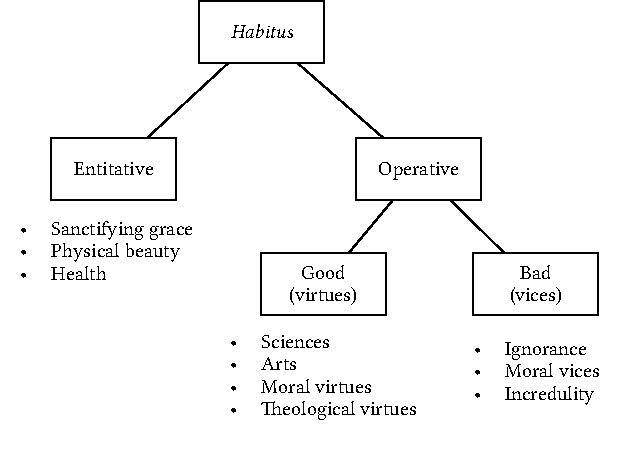
\includegraphics{images/habitus-examples-en.pdf}
    \caption{The divisions of \emph{habitus} and some examples of each.
    Note that dispositions are divided the same way as \emph{habitus},
    and, in fact, physical beauty and health are best described as
    dispositions. \label{fig:habitus-examples}}
    \end{figure}

    It is worth noting at this point some of the elements that operative
    \emph{habitus}\footnote{From now on, for brevity's sake I will speak
      only of \emph{habitus}, because that is the genus that logic falls
      under. However, all of these characteristics apply equally well to
      dispositions, unless otherwise specified. As we saw, dispositions
      are like \emph{habitus} in all respects, except for durability.}
    all have in common, many of which they share in common with
    faculties. In particular, both operative \emph{habitus} and
    faculties are inherent in a \emph{subject} or substrate, and both
    are principles or originators of \emph{operation}, and both have an
    \emph{object}, that is, the finality or term to which the operation
    is directed.

    As usual, it is helpful to look at examples. Let us look first of
    all at some faculties, starting with the faculty of sight. Like all
    faculties, the \emph{subject} (or \emph{substrate}) will be the
    substance in which it is inherent (in this case, an animal, rational
    or irrational). We can specify, however, that unlike purely
    immaterial faculties like the intellect, a sense like sight is
    dependent on the \emph{body} or \emph{matter} of the animal in
    question. The \emph{operation} that sight produces is called
    \emph{vision}, and the \emph{object} of sight can be described as
    \emph{material entities insofar as they have color}. Now, let us
    look at the human intellect. Being also a faculty, it will likewise
    have the substance as its \emph{subject} (in this case, the human
    being in question)---however, unlike the sense of sight, it stems
    directly from the human being's immaterial soul, with no dependence
    on the body for its existence. Its \emph{operations} include the
    simple apprehension of essences, and making judgments (mediated or
    immediate) regarding being. (We will return to this point in greater
    detail.) Its \emph{object} can be described as the entities it comes
    to know, insofar as they are intelligible (that is, insofar as they
    can be known in themselves).

    With operative \emph{habitus}, it is important to specify what we
    mean by \emph{subject}: like all accidents, operative \emph{habitus}
    inhere in the substance that they perfect, and so the substance
    could be regarded as their ``subject'' in that sense. However, more
    often, when we speak of the \emph{subject} of an operative
    \emph{habitus}, we mean the faculty that the \emph{habitus}
    modifies. That is the meaning that we will give the term in this
    introduction. Thus, for example, all the intellectual \emph{habitus}
    that we have talked about up to now---sciences and arts---have the
    intellect as their subject. If we look at, say, quantum mechanics,
    its \emph{object} is what the science studies: material entities as
    regards the behavior of the elemental particles that constitute
    them, and the \emph{operations} it produces consist in the acts of
    apprehending and judgment by the intellect regarding that object.
    Note that without the \emph{habitus} of quantum physics, such
    apprehensions and judgments would be impossible; thus, the habitus
    is a true principle, or origin, of operation, albeit a secondary one
    that depends on the intellect and ultimately on the substance (that
    is, the human being) in which it inheres.

    Similarly, if we look at an art---say, carpentry---the
    \emph{subject} is, of course, the intellect; the \emph{object} is
    the works of carpentry produced, which consists of pieces of wood to
    be shaped into tables, chairs, and the like; and the operations
    consist in the combination of knowhow and physical actions required
    to shape the wood into the products desired. Table
    \ref{tab:subject-operation-object} summarizes the examples we have
    just gone over, with some additions.

    \begin{table}[ht]
    \begin{center}
    \caption{The subject, operations, and object of various faculties and operative \emph{habitus}.}
    \label{tab:subject-operation-object}
    {
    \disablehyphenation
    \small
    \begin{tabular}{l|l|>{\raggedright}p{0.26\linewidth}|p{0.26\linewidth}}
    \toprule
     & Subject & Operation & Object \\
    \midrule
    Sight & Substance (body) & Vision & \emph{Ens} as colored \\ 
    Intellect & Substance (soul) & Apprehension, judgment & \emph{Ens} as intelligible \\
    Will & Substance (soul) & Desire, love & \emph{Ens} as desirable \\
    \midrule
    Quantum physics & Intellect & Apprehension, judgment (of Q.P.) & Material \emph{ens} as regards elementary particles \\
    \midrule
    Carpentry & Intellect & Actions to shape wood & Wood to be shaped \\
    \midrule
    Logic & Intellect & Apprehension, judgment, reasoning & Works of reason \\
    \bottomrule
    \end{tabular}
    }
    \end{center}
    \end{table}

    \hypertarget{operations}{%
    \subsection{Operations}\label{operations}}

    Of course, the effect of having faculties and \emph{habitus} is the
    capacity for \emph{operation} (Greek: ἐνέργεια, \emph{enérgeia}),
    which is simply the philosophical term for any actions that are
    produced by a substance. As we have seen, operations always have
    their \emph{ultimate} origin in the substance itself, but the
    faculty that produces them, together with any \emph{habitus} that
    perfects it, can rightly be considered the \emph{immediate} origins
    of that operation. In our oft-cited example, the scientist who
    contemplates Schrödinger's equation is rightly considered the author
    or origin of the act (operation) of contemplating. However, he
    engages in this operation by the mediation of his intellect, which
    has been perfected by the science of quantum physics (an operative
    \emph{habitus}).

    Figure \ref{fig:substance-operation} illustrates the hierarchical
    relationship among substance, faculty, \emph{habitus}, and
    operation. Operations can be produced entirely by the substance that
    acts, or else the substance may receive the power to act from an
    extrinsic source. For instance, an animal's capacity for locomotion
    is entirely intrinsic to itself; however, if it is trained to
    perform certain actions by a human master (say, for a dog to perform
    tricks or to sniff for contraband), it is acting based on training
    that it has received extrinsically. Similarly, a human being can do
    acts of knowledge and love under his own power; however, he can only
    do acts of supernatural knowledge (faith) and supernatural love
    (hope and charity) under the influence of sanctifying grace, which
    he receives from God. However, logic deals with the works of reason,
    which are the result of operations that are entirely intrinsic to
    man and do not require an extrinsic power. As shown in the diagram,
    all operations that are proper---that is, intrinsic---to the
    substance that produces them ultimately have their origin in the
    substance's \emph{actus essendi} or \emph{act of being}. This is a
    principle that you will learn about in your course on metaphysics:
    but for now, it is sufficient to say that it is a metaphysical
    principle that is the source of all proper actuality (i.e., all the
    actuality that does not come from outside) in a substance. The
    \emph{essence} (\emph{essentia}) signifies the substance inasmuch as
    it is a metaphysical principle, a capacity that it fulfills in two
    ways: as the substrate for the accidents, and as the potency
    receives the act of being. As such, the essence acts as a limit to
    and a measure of the intensity of the act of being. The first
    perfections to emanate from the substance are the active potencies
    (\emph{potentiae activae}), which, as we saw, include the faculties
    of sentient substances. Those faculties that entail a considerable
    freedom of action---especially the rational faculties in man---are
    further perfected by operative \emph{habitus}.

    Putting all this together, all operations emanate from the
    substance's \emph{actus essendi}. Those operations that are entirely
    intrinsic trace all of their actuality to this act of being; others
    require the assistance of an outside power. Regardless, operations
    are produced by the mediation of substance's active powers. In
    sentient and rational beings, some of these powers---called
    \emph{faculties}---are capable of a further perfection that we call
    operative \emph{habitus}. Thus, a substance's operations pass
    through, as it were, two and possibly three filters: the essence
    itself (which already sets certain limits to what kinds of
    operations are possible), the faculties that produce the operations,
    and, where this is possible, the \emph{habitus} that perfect the
    faculties.

    \begin{figure}
    \centering
    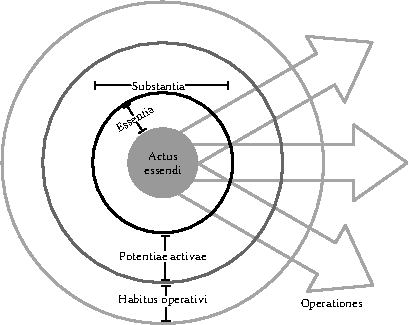
\includegraphics{images/substance-operation-graphic.pdf}
    \caption{An illustration how a substance produces operations.
    \label{fig:substance-operation}}
    \end{figure}

    \hypertarget{the-operations-of-the-intellect}{%
    \section{The Operations of the
    Intellect}\label{the-operations-of-the-intellect}}

    The object of this short primer on the metaphysics of man is, of
    course, to understand the three operations that most closely respect
    logic, that is, the operations of the intellect.
\end{document}
